\begin{strip}
\centering
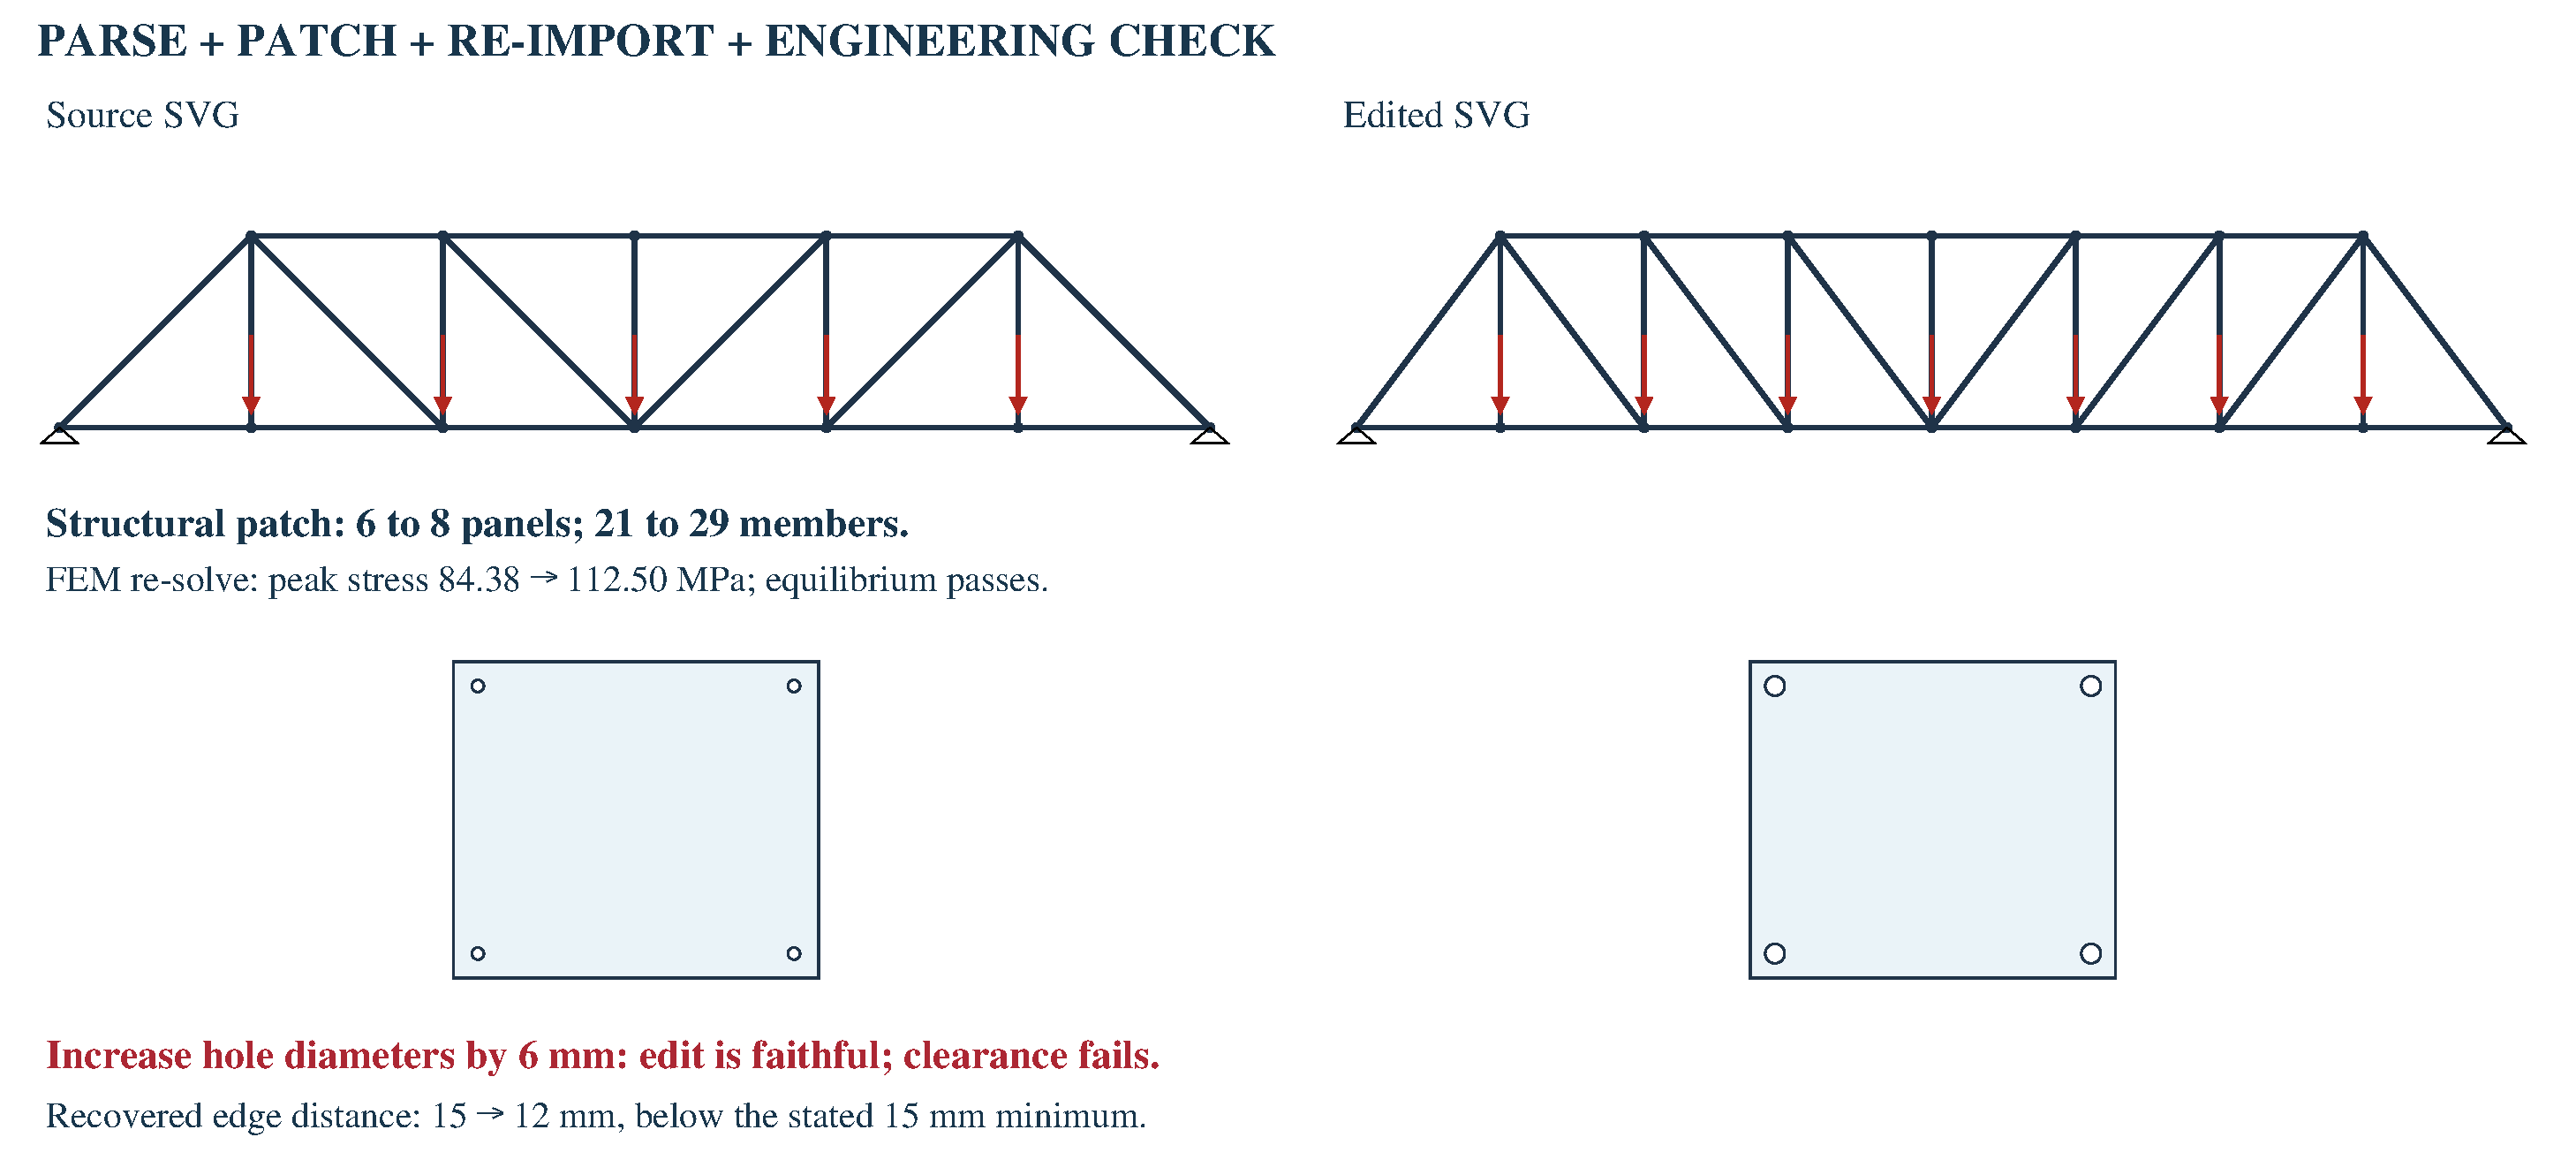
\includegraphics[width=\linewidth]{figures/editor-overview.pdf}
\captionsetup{hypcap=false}
\captionof{figure}{\textbf{Two edits, re-imported and re-checked.}
\textbf{Top:} ``Change the bridge to 8 panels'' on a Pratt truss with span $L{=}12$\,m, depth $h{=}2$\,m and
member area $A{=}800$\,mm$^2$ ($E{=}200$\,GPa). The 53-operation patch repositions 36 existing elements,
inserts 8 members, 4 joints and 2 load arrows, and updates the title, giving 29 members. The drawing specifies
$P{=}15$\,kN per loaded node, so the loaded bottom-chord nodes increase from 5 to 7 (total load 75\,$\to$\,105\,kN).
Axial FEM on the re-imported drawing gives a peak member stress of 84.4\,$\to$\,112.5\,MPa, equal to the midspan chord
force $PLn/(8h)$ divided by $A$ for $n{=}6\,{\to}\,8$ panels, and a peak displacement of 8.95\,$\to$\,11.85\,mm; the relative
equilibrium residual is below $10^{-13}$. This confirms that the edited truss is solvable and in equilibrium. No stress
limit is applied, so it does not show that the bridge is safe.
\textbf{Bottom:} ``Increase all hole diameters by 6\,mm'' on a 300$\times$260$\times$9\,mm plate whose hole centres lie
$c{=}20$\,mm from both adjacent edges. The two-operation patch changes $d$ from 10 to 16\,mm and updates the hole note,
matching the target SVG tree exactly. The clear edge distance $e{=}c-d/2$ falls from 15 to 12\,mm, below the 15\,mm minimum.
The source holes already sit at that minimum, so with fixed centres the rule allows only $d\le2(c-15)=10$\,mm;
16\,mm holes need $c\ge23$\,mm. The request is infeasible as stated: the editor applies it without moving the holes,
and the check reports the violation. This is a geometric clearance rule, not FEM. Geometry is cropped from the source
and edited SVGs, with labels omitted and colors normalized.}
\captionsetup{hypcap=true}
\label{fig:teaser}
\end{strip}
